\chapter{Protocols and Related Works}
\label{chap: Related works}

\textit{This chapter describes the attempts on Cryptography protocols behind the existing HD wallets as
    well as the attempt of adapting these mechanisms to curve Ed25519. We analyze the famous wallet that the community are using.}

\minitoc

\section{Related Protocol}
\subsection{Key Derivation}

The word “Hierarchical Deterministic” in crypto wallet were first introduced by Pieter Wuille in Bitcoin Improvement Proposal number 32 (BIP32)\cite{github/bip0032}. The initial idea was to build a wallet architect like a tree. From the root seed, we can derive child private keys and child public keys that construct many child wallets for different purposes. However, BIP32 only supports the elliptic curve used in Bitcoin, defined by the name ``secp256k1" \cite{secp256k1}. SatoshiLabs Improvement Proposal number 10 (SLIP10) is an attempt to generalize the BIP32's key derivation schema for different curves, e.g., NIST P-256 and Ed25519. For some security reasons, SLIP10 forbade normal child key derivation on curve Ed25519. But SLIP23 adopted them both and proposed a new schema on curve Edwards25519 called ``BIP32-Ed25519" \cite{Khovratovich2017}. In this section, we will explain how these schemes work and analyze the difficulties in adapting BIP32 to the Edwards25519 Curve.

\subsubsection{BIP32}
\label{bip32}
The most significant motivation of BIP32 is how one can calculate the public key of another without revealing the private keys or the sender has to generate it from private keys. Elliptic curve mathematics permits these kinds of schemes. For example, a webshop business lets its web server generate fresh addresses (public key hashes) for each order or for each customer, without giving the webserver access to the corresponding private keys (which are required for spending the received funds).

BIP32 also makes wallets more recoverable since users only have to maintain the root seed and a list of wallet indexes. In the example of a webshop, the web owner doesn’t have to keep all the private keys safe, and this becomes more redundant if the owner has an increase in a business requiring more wallets. Instead, he only has to create the seed one and save the indexes each time he makes a wallet. The next part will cover the indexes of children’ wallets and how we can recover the entire wallet structure using the initial seed and list of indexes.

\bigskip
{\textbf{Derivation}}. BIP 32 key derivation is a mechanism used to generate a specific ECDSA key pair within a tree of indexes. Given a parent extended key and an array of indexes, we will be able to deterministically regenerate keys at that specified index in the tree. Starting from a master seed to the creation of one master extended key, we can create a tree with infinite depth. Each node can also have a maximum of 4,294,967,296 child nodes (2³²/32-bit unsigned integer) resulting in an incredible ability to generate a limitless number of keys. \autoref{fig:bip32} is an example of a BIP32 key tree with depth 3.

\begin{figure}[ht!]
    \centering
    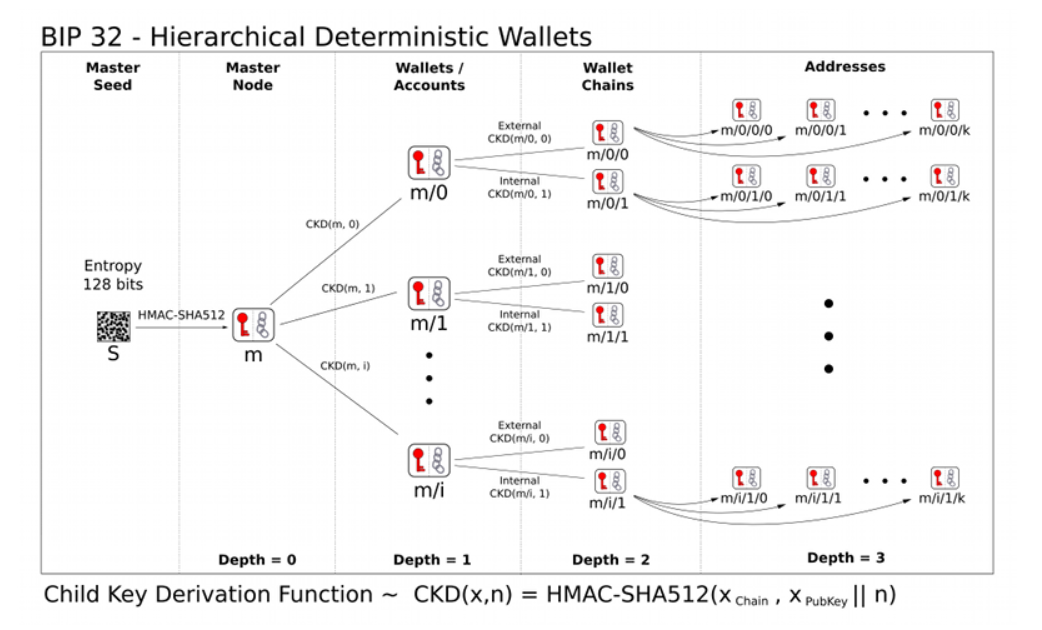
\includegraphics[width=1\textwidth]{images/bip32.png}
    \caption[Example of BIP32 key tree with depth 3]{Example of BIP32 key tree with depth 3 \cite{github/bip0032}}
    \label{fig:bip32}
\end{figure}


\bigskip
{\textbf{Extended keys}}. An extended key is defined as follow:

\begin{adjustwidth}{2cm}{}
    An extended key consists of a private or public key and chain code. An extended key can create children, generating its own branch in the tree structure. Sharing an extended key gives access to the entire branch.
\end{adjustwidth}

The term ``extended key" could also be thought of as ``extensible key" because such a key can be used to derive children. BIP32 extends both private and public keys first with an extra chain code. This extension is added in order to prevent depending solely on the key itself; it also is identical for corresponding private and public keys.

In total, an extended key is represented simply as the concatenation of the 32 bytes key and 32 bytes chain code into a 64 bytes sequence (512-bits). So the total number of possible extended key pairs is almost 2512, but the produced keys are only 256 bits long and offer about half of that in terms of security. But the designed key size already satisfies the requirement of the NIST recommendation. In specifically, to maintain security against classical attacks, NIST has recommended transitions from key sizes and algorithms that provide 80 bits of security to key sizes and algorithms that provide 112 or 128 bits of security in 2016 \cite{Barker2019}.

\begin{figure}[ht!]
    \centering
    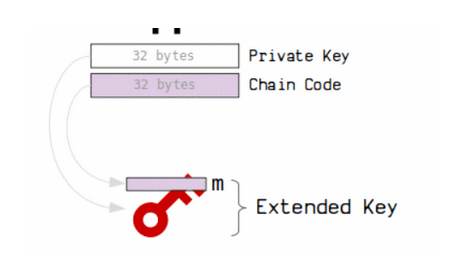
\includegraphics[width=0.7\textwidth]{images/extended_key.png}
    \caption[Example of the extended private key]{Example of the extended private key \cite{learnme}}
    \label{fig:extended_key}
\end{figure}

Driven by advances in both classical and quantum computing technologies, in May 2020, NIST recommended improving key length to 256 bits \cite{Barker2020}. It is unclear when scalable quantum computers will be available, and we will keep updating our system with the latest news on NIST publication.

Child key on the BIP32 key tree can only be derived from an extended key. From a security perspective, this is an excellent idea on how we can protect the child keys if the attackers get a hold of a stolen parent key. Because the extended key is collectively made up of a combination of key and chain code, attackers won’t have a better way to derive the children keys other than brute-forcing 32 bytes of extended entropy.

There are two types of extended keys. An extended private key is the combination of a private key and chain code and can be used to derive child private keys (and from them, child public keys) (see \autoref{fig:extended_key}). An extended public key is a public key and chain code, which can be used to create child public keys (public only).

The index of the child key is a 32-bit integer, meaning that each extended key has $2^{32}$ child keys. This index number is divided into two ranges to easily determine between keys derived through the normal derivation function versus keys derived from hardened derivation. Index numbers between 0 and $2^{31}$–1 (0x0 to 0x7FFFFFFF) are used for normal derivation and the index numbers between $2^{31}$ and $2^{32}$–1 (0x80000000 to 0xFFFFFFFF) are used only for hardened derivation. Therefore, the normal child will have an index of less than $2^{31}$, whereas the hardened child index equals or is above  $2^{31}$.

We couldn’t find any reason behind why the author of BIP32 designed the parent extended keys to have $2^{32}$ total child keys each. Poulami Das et al.\cite{DBLP:conf/ccs/0003EFL021} investigated BIP32 with security analysis and experimented with a similar key derivation schema (BIP32-m) with only $2^{20}$ child keys, pointing out $2^{32}$ child keys won’t create any vulnerability on the system.

In the next part, we will represent an extended private key as $(k, c)$, with $k$ the normal private key, and $c$ the chain code. An extended public key is represented as $(K, c)$, with $K = point(k)$ and $c$ the chain code. The index is denoted to \textit{i}; to ease, $i_H$ is the index of a hardened key representing a number of $i+2^{31}$.

\bigskip
{\textbf{Convention}}. In the rest of this thesis, we will assume the public key cryptography used in Blockchain, namely elliptic curve cryptography using the field and curve parameters. Variables below are either:

\begin{itemize}
    \item Integers modulo the order of the curve (referred to as $n$).

    \item Coordinates of points on the curve.

    \item Byte sequences.
\end{itemize}

The addition (+) of two coordinate pairs is defined as the application of the EC group operation. Concatenation ($\parallel$) is the operation of appending one-byte sequence onto another.

As standard conversion functions, we assume:

\begin{itemize}
    \item $point(p)$: returns the coordinate pair resulting from EC point multiplication (repeated application of the EC group operation) of base point with the integer $p$.

    \item $ser_{32}(i)$: serialize a 32-bit unsigned integer $i$ as a 4-byte sequence, most significant byte first.

    \item $ser_{256}(p)$: serializes the integer $p$ as a 32-byte sequence, most significant byte first.
    \item $ser_P(P)$: serializes the coordinate pair $P = (x,y)$ as a byte sequence using the compressed form: $(0x02$ or $0x03) \parallel ser_{256}(x)$, where the header byte depends on the parity of the omitted $y$ coordinate. 0x02 if $y$ is positive and 0x03 if $y$ is negative.
    \item $parse_{256}(p)$: interprets a 32-byte sequence as a 256-bit number, most significant byte first.
\end{itemize}


\bigskip
{\textbf{Master Extended Key generation function}}. Master extended key is the first key to be generated from the root seed. A master key also possesses a size of $2^{512}$ where 256 first bits is the master private key and the last 256 bits is the chain code. From the master private key, we can calculate the master public key.

\begin{figure}[ht!]
    \centering
    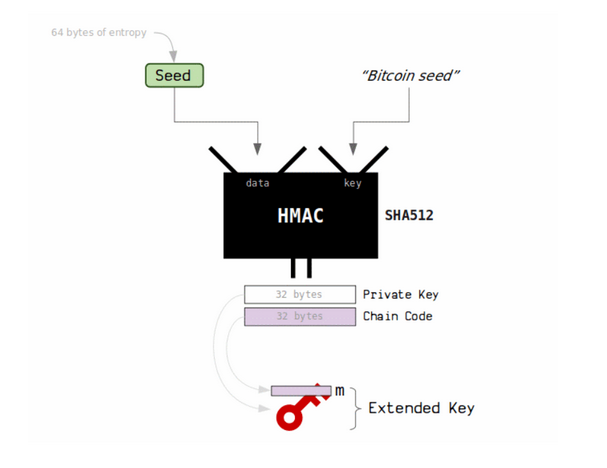
\includegraphics[width=0.9\textwidth]{images/masterbip32.png}
    \caption[Master Extended Key generation Process]{Master Extended Key generation Process \cite{learnme}}
    \label{fig:master_bip32}
\end{figure}

Pseudo-code of generation function is as below:

\begin{enumerate}
    \item Generate a seed byte sequence $S$ of a chosen length (between 128 and 512 bits; 256 bits is advised) from a (pseudo) random number generator (PRNG).

          \begin{quote}
              The PRNG, as mentioned in Section \ref{chap:background}, is recommended to produce a root seed. However, BIP39 \cite{github/bip0039} invented a method to create a seed from mnemonic code or mnemonic sentence entropy. We will discuss BIP39 in Section \ref{SLIP10} . Ideally, the creation of BIP39 helps users to maintain their wallets more efficiently since secure random sentences (12 to 24 words) are more comfortable than protecting a random byte sequence.
          \end{quote}

    \item Calculate $I$ = HMAC-SHA512(Key = ``Bitcoin seed", Data = $S$)
          \begin{quote}
              The HMAC function returns 512 bits of data (which is totally unpredictable) from a key and data component. BIP32 added the key ``Bitcoin seed" to the function, although it could be arbitrary when deriving the master node from the seed. This is considered necessary to ensure proper domain separation between different elliptic curves or different types of key hierarchy generation schemas.
          \end{quote}

    \item Split $I$ into two 32-byte sequences, $I_L$ and $I_R$.

          \begin{quote}
              The result of the HMAC function with the size 512 bits (64 bytes) will be split into 32 bits left  $I_L$ and 32 bits right $I_R$.
          \end{quote}
    \item Use $parse_{256}(I_L)$ as the master secret key, and $I_R$ as master chain code.

          \begin{quote}
              Return 32 bits left $I_L$ as the secret key and 32 bits right $I_R$ as the extended chain code.
          \end{quote}

\end{enumerate}
In case $I_L$ is 0 or $n$ (private key  order $n$), the master key is invalid.

\bigskip

\textbf{Discussing the function HMAC-SHA512}. The HMAC-SHA512 is specified in \cite{Nystrom2005}. It is used in all key derivation functions of the BIP32 schema.
This raises the question: isn't it just SHA512 with the input as Key $\parallel$ data is enough to generate an unexpected output of the root seed? We believe the answer is to avoid the
flaws that can be caused by simple concatenation, for example length extention attacks. In cryptography and computer security, a length extension attack is a type of attack where an attacker can use Hash(message1) and the length of message1 to calculate Hash(message1 ‖ message2) for an attacker-controlled message2, without needing to know the content of message1.
Also it provide a better integrity of information for the secret keys.


\bigskip
{\textbf{Child key derivation (CKD) functions}}. There are 3 methods for deriving child keys:
\begin{enumerate}
    \item Private parent key $\rightarrow$ normal private child key;
    \item Public parent key $\rightarrow$ normal public child key;
    \item Private parent key $\rightarrow$ hardened private child key;
\end{enumerate}
And public parent key $\rightarrow$ private child key is not possible. Derived child extended keys (and parent keys) are independent of each other. In other words, you wouldn’t know that two public keys in an extended tree are connected in any way.

\bigskip
{\textbf{Normal extended child private key derivation function}}.\label{norm1} The function CKDpriv(($k_{par}$, $c_{par}$), $i$) $\rightarrow$ ($k_i$, $c_i$) computes a normal child extended private key from the parent extended key.
The \autoref{fig:1} describes the process.

\begin{figure}[ht!]
    \centering
    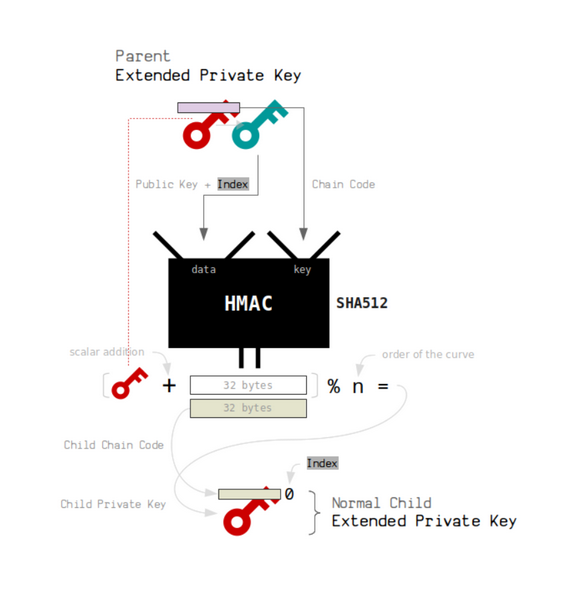
\includegraphics[width=0.9\textwidth]{images/normal_extended_private_gen.png}
    \caption[Normal Extended Private Key generation process]{Normal Extended Private Key generation process \cite{learnme}}
    \label{fig:1}
\end{figure}

Pseudo-code:
\begin{enumerate}
    \item Check whether $i \geq 2^{31}$ (whether the child is a hardened key).
          \begin{itemize}
              \item If so (hardened child): return false

              \item If not (normal child):
                    \begin{quote}

                        Let $I$ = HMAC-SHA512(Key = $c_{par}$, Data = $ser_P(point(k_{par}))$ $\parallel$ $ser_{32}(i)$).
                        Key input $c_{par}$ is the chain code of the extended parent key. Data input $ser_P(point(k_{par}))$ $\parallel$ $ser_{32}(i)$ contains 2 parts that are concatenated together. The $point(k_{par}$) is the result of working out the coordinate pair of the public key from $k_{par}$, as shown in Figure 4, the public parent is a part of the Data. The function $ser_{P}$ will return the compressed representation of $point(k_{par}$) with the size of 33 bytes \cite{secp256k1}. And the value $ser_{32}(i)$ is just the representation of the normal index—two of these elements concatenated together to form the data of HMAC-SHA512 function.
                    \end{quote}

          \end{itemize}
          \bigskip

    \item Split $I$ into two 32-byte sequences, $I_L$ and $I_R$.
          \bigskip

    \item The returned child key $k_i$ is $parse_{256}(I_L)$ + $k_{par}$ (mod $n$).

          \begin{quote}
              The child $k_i$ is an increment of the private parent key $k_{par}$ with the amount of $parse_{256}(I_L)$. We take the module of the new private key by the order of the curve ($n$) to keep the new private key belonging to the valid range of numbers for the secp256k1 curve. As mentioned previously, a very useful characteristic of BIP32 wallets is the ability to derive public child keys from public parent keys, without having the private keys. This returned key plays an important part in that ability.
          \end{quote}
          \bigskip

    \item The returned chain code $c_i$ is $I_R$.
          \bigskip

    \item In case $parse_{256}(I_L)$ $\geq$ $n$ or $k_i$ = 0, the resulting key is invalid, and one should proceed with the next value for i. (Note: this has probability lower than 1 in $2^{127}$.)

\end{enumerate}

To summarize, we make use of the data contained inside the parent extended private key: the private key, the chain code, and the index of the desired child. Putting it through the HMAC function will generate some unique random bytes. We use these new random bytes to construct the following private key from the old one.

\bigskip
{\textbf{Normal extended child private key derivation function}}. \label{norm2}The function CKDpub(($K_{par}$, $c_{par}$), i) $\rightarrow$ ($K_i$, $c_i$) computes a child extended public key from the parent extended key. It is only defined for non-hardened child keys.
The \autoref{fig:2} describes the process.

\begin{figure}[ht!]
    \centering
    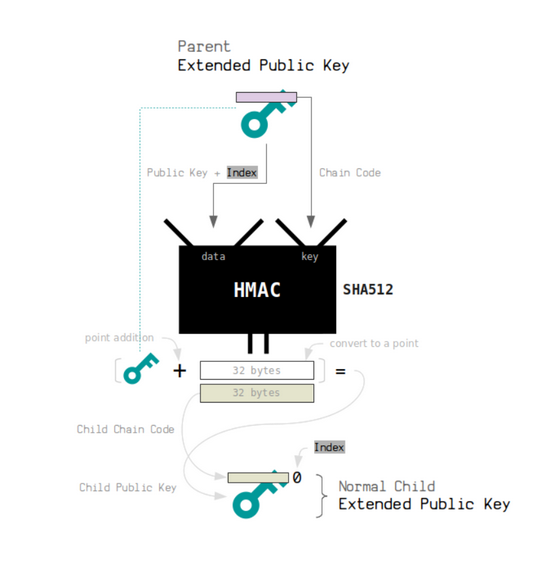
\includegraphics[width=0.9\textwidth]{images/normal_pub_gen.png}
    \caption[Normal Extended Public Key generation process]{Normal Extended Public Key generation process \cite{learnme}}
    \label{fig:2}
\end{figure}

Pseudo-code:
\begin{enumerate}
    \item Check whether $i \geq 2^{31}$ (whether the child is a hardened key).
          \begin{itemize}
              \item If so (hardened child): return false

              \item If not (normal child):
                    \begin{quote}

                        Let $I$ = HMAC-SHA512(Key = $c_{par}$, Data = $ser_{P}(K_{par})$ $\parallel$ $ser_{32}(i)$).
                        The function $ser_{P}(K_{par})$ returns the compressed representation of the parent public key with the size of 33 bytes. And the value $ser_{32}(i)$ is just the representation of the normal index.
                    \end{quote}
          \end{itemize}
          \bigskip

    \item Split $I$ into two 32-byte sequences, $I_L$ and $I_R$.
          \bigskip

    \item The returned child key $K_i$ is $point(parse_{256}(I_L))$ + $K_{par}$.

          \begin{quote}
              The split left half $I_L$ will be converted into a point on curve secp256k1 by function $point()$. Then $point(parse_{256}(I_L))$ + $K_{par}$ is the point addition on curve secp256k1 and returns the child public key.
          \end{quote}
          \bigskip

    \item In case $parse_{256}(I_L)$ $\geq$ n or $K_i$ is the point at infinity, the resulting key is invalid, and one should proceed with the next value for i.

\end{enumerate}

In summary, public key derivation only allows normal child derivation.
Putting the same key and Data through the HMAC function as we did in normal private, we can produce the child public key from the left 32 bytes via elliptic curve point addition.
The schema normal key derivation make the motivation of BIP32 come true. We will explain the relation between normal keys derivation.
It is very convenient to derive a branch of public keys from an extended parent key, but it comes with a potential key leakage.
We will discuss the potential risk of normal child key derivation schema compared to its value in the very last of this Section and analyze if it is suitable for our thesis.


\bigskip
{\textbf{Hardened extended child private key derivation function}}. The function CKDpriv(($k_{par}$, $c_{par}$), i) → ($k_i$, $c_i$) computes a child extended private key from the parent extended key.
The \autoref{fig:3} describes the process.

\begin{figure}[ht!]
    \centering
    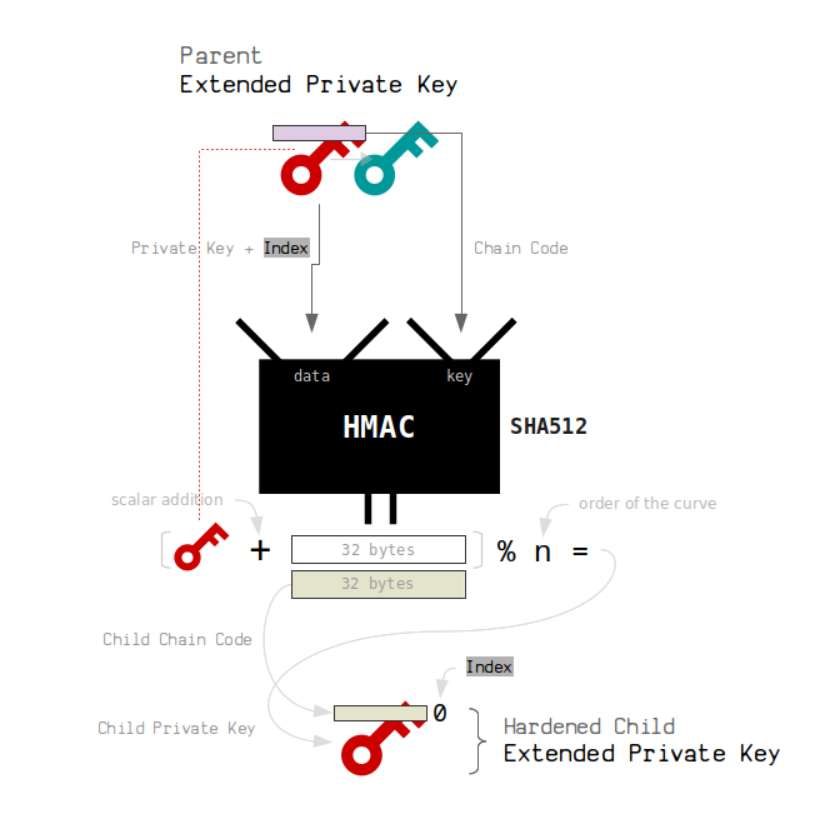
\includegraphics[width=0.9\textwidth]{images/hard_private_gen.png}
    \caption[Hardened Extended Private Key generation process]{Hardened Extended Private Key generation process \cite{learnme}}
    \label{fig:3}
\end{figure}

Pseudo-code:

\begin{enumerate}
    \item Check whether $i \geq 2^{31}$ (whether the child is a hardened key).
          \begin{itemize}
              \item If so (hardened child):
                    \begin{quote}

                        Let $I$ = HMAC-SHA512(Key = $c_{par}$, Data = 0x00 $\parallel$ $ser_{256}(k_{par}$) $\parallel$ $ser_{32}(i)$). (Note: The 0x00 pads the private key to make it 33 bytes long.)

                        The difference in hardened key derivation is that we don't recover the public key from the parent extended key. Instead, we padded 0 to the left of $k_{par}$ to make it 33 bytes long. Adding the leading zeros will not change the value. However, it is needed, so the number takes up the entire 33 bytes. (Since the compressed representation of a public key is 33 bytes).
                    \end{quote}


              \item If not (normal child): return false

          \end{itemize}
          \bigskip

    \item Split $I$ into two 32-byte sequences, $I_L$ and $I_R$.
          \bigskip

    \item The returned child key $k_i$ is $parse_{256}(I_L)$ + $k_{par}$ (mod $n$).
          \bigskip

    \item The returned chain code $c_i$ is $I_R$.
          \bigskip

    \item In case $parse_{256}(I_L)$ $\geq$ n or $k_i$ = 0, the resulting key is invalid, and one should proceed with the next value for $i$. (Note: this has probability lower than 1 in $2^{127}$.)

\end{enumerate}

The hardened derivation is therefore used to create a ``gap" in the tree above the level where extended public keys are used. Therefore, The hardened key derivation schema is needed to preserve security in HD Wallet.

\bigskip
{\textbf{The relation between normal keys derivation}}. From here to the rest of BIP32 section, we assume a scenario where:
\begin{quote}
    Alice is a shop owner, and she wants to create an HD wallet. Each wallet can receive and transfer coins for different purposes. She decided to use a wallet with the normal key derivation schema to transfer money between her wallet and others without any private key access whatsoever.

    Bob wants to transfer 1 Bitcoin to Alice. He generates an address from Alice's master public key and chain code using normal child key derivation schema with an index $i$. Bob sends 1 Bitcoin to that address with the message containing the index $i$.

    Alice now can generate the normal child private key from the master secret key with an index $i$ and possess a child wallet with an index $i$.

\end{quote}

What Bob just did is derive a public key from the master extended public key that corresponds to the Alice private key derived from Alice’s master extended private key, without knowing her extended private key. This scenario comes to reality thanks to the point addition law of the elliptic curve.

Denote child private key is $k_{child}$, child public key is $K_{child}$. From normal extended child private key derivation function, we have:

\begin{itemize}
    \item $I$ = HMAC-SHA512(Key = $c_{par}$, Data = $ser_P(point(k_{par}))$ $\parallel$ $ser_{32}(i)$)
    \item Child private key $k_{child}$ = $parse_{256}(I[:32])$ +  $k_{par}$ (mod $n$).
\end{itemize}

and normal extended child public key derivation function, we have:
\begin{itemize}
    \item $I$ = HMAC-SHA512(Key = $c_{par}$, Data = $ser_{P}(K_{par})$ $\parallel$ $ser_{32}(i)$).
    \item Child public key $K_{child}$ = $point(parse_{256}(I[:32]))$ + $K_{par}$.
\end{itemize}

For both child extended keys, we are inserting the \textit{identical inputs} to the HMAC function. The Key is the parent chain code. The Data is the parent public key. Through the HMAC function, we generate the same data as a result. Using the left 32 bytes of this result, we calculate:
\begin{itemize}
    \item Increase the parent private key $k_{par}$ an amount of the same 32 bytes (which is a number) to get the $k_{child}$.

    \item Apply point addition on the parent public key $K_{par}$ by the same 32 bytes to create the child public key $K_{child}$.
\end{itemize}

On account of the mechanism elliptic curve mathematics works, the derived child private key will correspond to the derived child public key:

\begin{equation}
    (k_{par} + I[:32]) . G  =  k_{child} . G =  K_{child}.
\end{equation}

\bigskip
\begin{figure}[ht!]
    \centering
    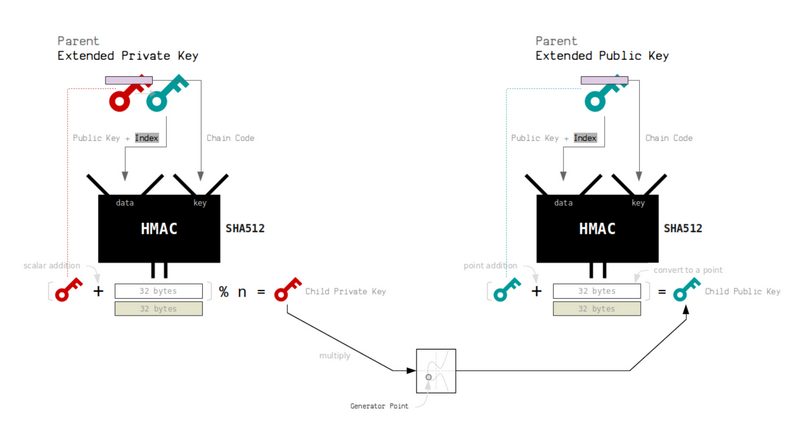
\includegraphics[width=1\textwidth]{images/relation_bip32.png}
    \caption[Relation in BIP32 normal derivation protocol]{Relation in BIP32 normal derivation protocol \cite{learnme}}
    \label{fig:4}
\end{figure}

\autoref{fig:4} presents the relation of normal derived child keys with their parent keys.

\bigskip
{\textbf{Discuss the potential risk of normal child key derivation schema}}
\label{bip32vul}
\begin{adjustwidth}{1cm}{}
    \bigskip
    {\textbf{First, the value}}. This shortcut can be used to create a very secure public key–only deployments where a server or application has a copy of an extended public key and no private keys whatsoever. That kind of deployment can produce an infinite number of public keys and Bitcoin addresses, but cannot spend any of the money sent to those addresses. Meanwhile, on another, more secure server, the extended private key can derive all the corresponding private keys to sign transactions and spend the money.

    One common application of this solution is to install an extended public key on a web server that serves an eCommerce application. The web server can use the public key derivation function to create a new Bitcoin address for every transaction (e.g., for a customer shopping cart). The web server will not have any private keys that would be vulnerable to theft. Without HD wallets, the only way to do this is to generate thousands of Bitcoin addresses on a separate secure server and then preload them on the eCommerce server. That approach is cumbersome and requires constant maintenance to ensure that the eCommerce server doesn’t ``run out" of addresses.

    Another common application of this solution is for cold storage or hardware wallets. In that scenario, the extended private key can be stored on a paper wallet or hardware device (such as a Trezor hardware wallet), while the extended public key can be kept online. The user can create ``receive" addresses at will, while the private keys are safely stored offline. To spend the funds, the user can use the extended private key on an offline signing Bitcoin client or sign transactions on the hardware wallet device (e.g., Trezor).

    The main use case for which this feature is advertised is in hierarchical organizations: the treasurer of a company might have control over the root private key of a BIP32 wallet and then hand off a “child” seed to each of the company’s departments who will then use that seed to operate their own wallet. The treasurer will have the master key to everything, but each department will only have the key to their own part of the funds.

    \bigskip
    {\textbf{Second, the vulnerability}}. Gus Gutoski et al.\cite{DBLP:conf/fc/GutoskiS15} investigated the BIP32 schema and considered the normal derivation vulnerable to master key recovery attacks. This attack vector is well known in the Bitcoin community and is considered to be “cannot be avoided” for BIP32 HD Wallet. The whole wallet hierarchy can be exposed to the hackers if one of the child private key is leaked.

    Following Vitalik Buterin’s article \cite{Vitalik}, the hackers can generate the parent key of the leaked wallet if they can get their hands on the private child key ki. The formula to calculate $k_{par}$ is as follow:

    \begin{equation}
        k_i  = k_{par} + hash(K_{par}, c_{par}, i)
    \end{equation}
    \begin{equation}
        k_{par} = k_i - hash(K_{par}, c_{par}, i)
    \end{equation}

    \bigskip
    If the attackers already have users private keys, they are more likely to possess the index i as well, even if they are not, they can still brute force the index (range 0 to $2^{31}$) until satisfied the K(i) = k(i) * G. So that they can easily produce the parent private key. Not only that, together with a parent chain code, if they were continuing to perform the formula, they can reveal the master secret key. Worse, the master secret key with it’s chain code will generate the entire private keys of all the wallets.

    \bigskip
    {\textbf{Avoiding the weakness}}. The ability to derive a branch of public keys from an extended public key is advantageous, but it comes with the above potential risk. The more keys derived for each party lead to the more fragile their wallet becomes. In practice, we see a lot of HD wallets still use normal key derivation like (\href{https://electrum.org/#home}{Electrum lightweight Bitcoin Wallet}). We evaluate these kinds of wallets in Section \ref{related}. Right now, we consider those applications that use normal key derivation that their security limitations are well worth the benefit.

    To counter this risk, BIP32 later came up with hardened key derivation. The method is basically the same but does not evolve the parent public key to the input of HMAC function, which breaks the relation between parent public key $K_{par}$ and the child chain code (last 32 bytes). The hardened derivation function uses the parent private key to derive the child chain code instead of the parent public key. This creates a ``firewall" in the parent/child sequence, with a chain code that cannot be used to compromise a parent or sibling private key. When the hardened private derivation function is used, the resulting child private key and chain code are entirely different from what would result from the normal derivation function. The resulting keys can be used to produce extended public keys that are not vulnerable because they cannot exploit the chain code to reveal any private keys. Therefore, the hardened derivation is used to create a ``gap" in the tree above the level where extended public keys are used.

    In simple terms, if we want to avoid the risks, we can use a hardened derivation schema rather than a normal derivation. But the value of BIP32 is too great if we can apply it to our Edwards25519 curve. In Section \ref{bip32ed25519}, we will introduce the BIP32-Edwards25519 schema where normal derivation key leakage can totally be prevented but it also has flaws. For the next section, we present a schema of Edwards25519 key derivation, which is a part of an attempt to apply BIP32 globally.
\end{adjustwidth}

\subsubsection{SLIP10}
\label{SLIP10}

Due to the emergence of Blockchain technology and the more powerful full quantum attack, the industry applies some other more powerful curves and digital signature algorithms. The SatoshiLabs Improvement Proposals number 10 (SLIP10) \cite{github/slip0010} was created for this reason. It defines a new hierarchical key derivation schema which is an extended superset of the BIP32 derivation algorithm to work on other curves. With secp256k1, SLIP10 is basically compatible. For the sake of our thesis, we will only examine their adaptation for the curve Edwards25519.

\bigskip
{\textbf{Master key generation function}}. Adapting the master key generation from BIP32, SLIP10 also has a master key that possesses a size of 512 bits. From the master private key, we can calculate the master public key.
\autoref{fig:5} describes the process.

\bigskip
\begin{figure}[ht!]
    \centering
    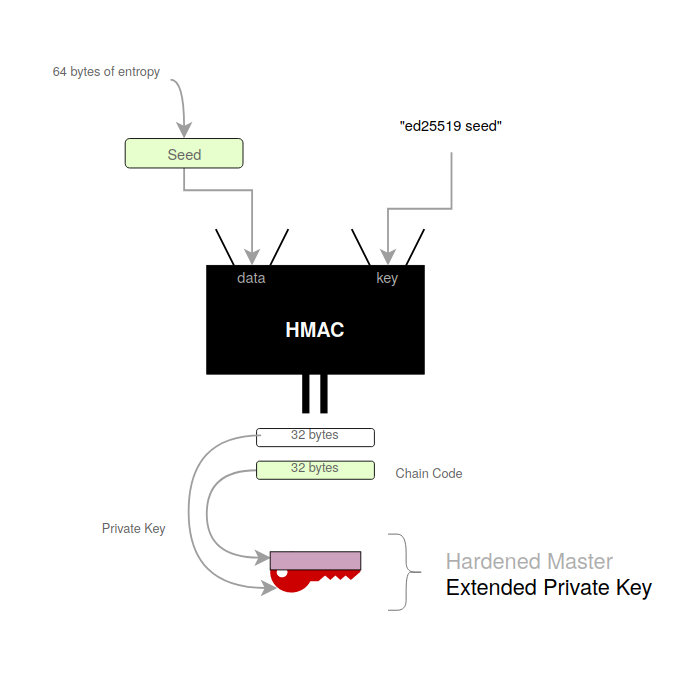
\includegraphics[width=1\textwidth]{images/master_slip10.png}
    \caption[Master Extended Key generation Process]{Master Extended Key generation Process}
    \label{fig:5}
\end{figure}

Pseudo-code:

\begin{enumerate}
    \item Calculate $I$ = HMAC-SHA512(Key = “ed25519 seed”, Data = $S$)

          \begin{quote}
              Random seed $S$ is a seed byte sequence of 128 to 512 bits in length (same as BIP32). The value of $S$ should be the binary seed obtained from a PRNG function, or it should be the master secret obtained from a set of BIPs39 mnemonic codes and arbitrary passphrases. BIP39 is also a part of the HD wallet, and we will introduce it in Section \ref{bip39}. For the Key input, we use “ed25519 seed” to avoid generating the same private key for different elliptic curves with different orders.
          \end{quote}

          \bigskip

    \item Split $I$ into two 32-byte sequences, $I_L$ and $I_R$.
          \bigskip

    \item Use $parse_{256}(I_L)$ as the master secret key, and $I_R$ as master chain code.

          \begin{quote}
              Because every 256-bit number (even 0) is a valid private key (see \ref{chap:background}) on curve Ed25519, we don’t have to validate the $parse_{256}(I_L)$ and return it as a secret key.
          \end{quote}
\end{enumerate}

\bigskip
{\textbf{Hardened child key derivation function}}. SLIP10 only supports hardened key generation for the Edwards25519 curve, meaning that we can not derive public child keys from any extended parent keys.

The function CKDpriv(($k_{par}$, $c_{par}$), $i$) → ($k_i$, $c_i$) computes a child extended private key from the parent extended private key. \autoref{fig:6} describes the process.

\bigskip
\begin{figure}[ht!]
    \centering
    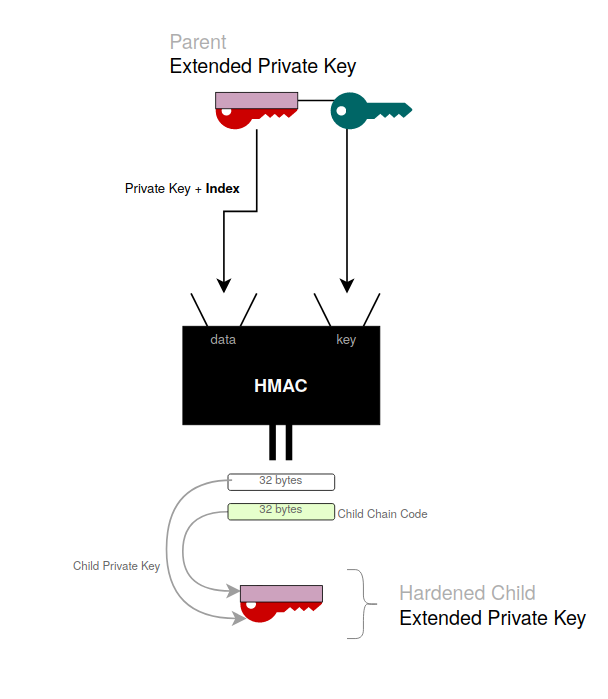
\includegraphics[width=0.9\textwidth]{images/hard_child_slip10.png}
    \caption[Hardened Extended Public Key generation process]{Hardened Extended Public Key generation process}
    \label{fig:6}
\end{figure}

Pseudo-code:
\begin{enumerate}
    \item Check whether $i \geq 2^{31}$ (whether the child is a hardened key).
          \begin{itemize}
              \item If so (hardened child):
                    \begin{quote}

                        Let $I$ = HMAC-SHA512(Key = $c_{par}$, Data = 0x00 $\parallel$ $ser_{256}(k_{par}$) $\parallel$ $ser_{32}(i)$). (Note: The 0x00 pads the private key to make it 33 bytes long.)

                        The return $I$ in SLIP10 is compatible with BIP32.
                    \end{quote}

              \item If not (normal child): return false

          \end{itemize}
          \bigskip

    \item Split $I$ into two 32-byte sequences, $I_L$ and $I_R$.
          \bigskip

    \item The returned chain code  $c_i$is $I_R$ and returned child key $k_i$ is $parse_{256}(I_L)$.
          \begin{quote}
              Same as the Master key generation function, SLIP10 returns the hashes directly as extended private child keys.
          \end{quote}
\end{enumerate}

The HMAC-SHA512 function is specified in the Background.

\bigskip
{\textbf{Difficulties in adapting BIP32 to Ed25519 curve}}. BIP32 was designed for curve secp256k1 only. Applying different curve schema is very challenging due to the nature of each curve. Ed25519 specifically, researchers around the world meet two main problems as below.


\begin{adjustwidth}{1cm}{}
    \bigskip
    {\textbf{Ed25519's private key is not the multipliers}}. Ed25519 key pair generation is different from secp256k1. \autoref{fig:multiply_ed25519} shows how public key A was generated from private key k. As we present in Section \ref{blockchain}, the public key A is the encoding of the point caused by a fixed-base scalar multiplication [s]B (B is the generator) where s is a “bit-clamping” (or pruning) value produced from the left half of the HMAC function result. The linearity in the BIP32 schema is lost entirely when applied to the Ed25519 keypair. The private keys are now no longer multipliers for the group generator.

    So the normal private keys, when derived, won’t correspond to the normal public key. The modified hash of the private key is now the multiplier. This cannot be changed since it is the core of speeding up in the Ed25519 curve. Researchers will have to find out another way to work around key derivation for Ed25519 because of this problem.

    \bigskip
    \begin{figure}[ht!]
        \centering
        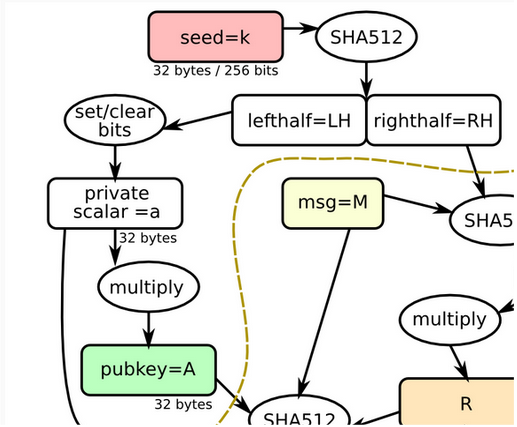
\includegraphics[width=0.9\textwidth]{images/ed25519_generator_multiplier.png}
        \caption[Multiply process of Ed25519]{Multiply process of Ed25519 \cite{learnme}}
        \label{fig:multiply_ed25519}
    \end{figure}


    \bigskip
    {\textbf{Ed25519's “bit clamping" problem}}. For performance reasons, Ed25519 doesn't provide a prime-order group and provides a group of order h * l instead, where h is a small cofactor of 8 and l is a 252-bit prime (Section \ref{cryptography}). In short, a cofactor is one of the parameters that make up an elliptic curve. The number of points on the elliptic curve can be described as n = r * h where r is the prime order of a subgroup and h is the cofactor.

    The method of using a cofactor to boost a better performance \cite{DBLP:journals/iacr/BernsteinL17} has proven to be a source of issues and vulnerabilities in higher-layer protocol. If the cofactor is 1, like in many of the standardized curves, it’s not something we need to worry about. If it is not one, careful consideration needs to be made for its implications in cryptographic schemes to avoid a few types of attacks, notably small-subgroup attacks \cite{DBLP:journals/rfc/rfc2785} and more announced malleability attacks (For example in Monero Blockchain \cite{Riccardo}).

    To prevent this, Ed25519 performs a “bit clamping” on step \textit{set/clear bits} in \autoref{fig:multiply_ed25519} as follow (bytes represented in little-endian form):

    \begin{itemize}
        \item input[0] \&= 248
              \begin{quote}
                  Setting the lowest 3 bits to 0 makes the private key the multiple of 8. This is only useful to prevent small-subgroup attacks in Diffie Hellman key exchange \cite{enwiki:1057850165}, but the creator of Ed25519 makes it a global schema. In our thesis, we don't use DH in any of our processes, so we won't discuss this problem further. Clearing these 3 bits does not roughly reduce the keyspace since it still leaves 252 higher bits, but if we continue to clamp through the process, this will result in big security issues (see Section \ref{bip32ed25519}).

              \end{quote}

              \bigskip

        \item The highest bit of the last byte is cleared, and the second-highest bit of the last byte is set to 1.
              \begin{quote}

                  Gregory Maxwell (Bitcoin core dev, CEO of Blockstream) said it would prevent the scalar from exceeding the order of the group \cite{mail:000860}. Furthermore, it's also a performance hack so that the exponentiation ladder does not need to correctly handle the point at infinity.

                  Later on, Daniel J. Bernstein (djb), the creator of Ed25519, explained in a mailing list post from 2014 that some implementations implement it in variable-time based on the position of the highest bit. To avoid implementations having to care about this, he decided to make this part of the standard so that if the implementation is variable time in that way, it will run in constant time because of this clamping \cite{Bernstein:2014}. This prevents side-channel attack vector via timing leakage on weak scalar multiplication implementations \cite{DBLP:journals/iacr/BrumleyT11}.

              \end{quote}

    \end{itemize}
    In conclusion, pruning the scalar generated from the private key changes the linearity of the system completely. SLIP10 avoids these issues because it doesn't try to support non-hardened parent public key to child public key derivation and only supports hardened private parent key to private child key derivation when used with the Ed25519 curve. Also, SLIP10 doesn't use any hardened derivation containing ``bit clamping" in the process. The randomly generated child keys act as a seed in the next generation. In the signature generation, they don't have to prune the secret key the second time. SLIP10 remains the most implemented key derivation structure that the blockchain community uses and is recommended to use.

\end{adjustwidth}


\subsubsection{SLIP23}
\label{bip32ed25519}

SatoshiLabs Improvement Proposals number 23 (SLIP23) is about Cardano HD master node derivation from a master seed, but also documented child key derivation function, which is based on Dmitry’s paper BIP32-Ed25519 \cite{Khovratovich2017}. We use SLIP23 instead of CIP03 (Cardano Improvement Proposal) because CIP is merely to document the existing standards and not to provide rationales for the various methods used in key derivation. For a long time, Cardano hasn’t updated documentation on this topic. Documentation about BIP32-Ed25519 on the Cardano website is also removed. This section describes a hierarchical deterministic key derivation approach for curve Ed25519 that overcomes the security issues mentioned in BIP32.

In practice, there is much confusion in implementing the original paper to their library (or application). In every next part, we will present the most general ideas of the original paper.

\bigskip
{\textbf{Master Extended Key generation function (root key in the paper)}}. This scheme adopts the master node derivation used in BIP32 and SLIP10 but defines a new Key input ``Ed25519 cardano seed" for the Cardano deterministic key hierarchy. They implement ed25519's ``bit clamping" to the derivation schema.

\autoref{fig:slip23_master} describes the process.

\begin{figure}[ht!]
    \centering
    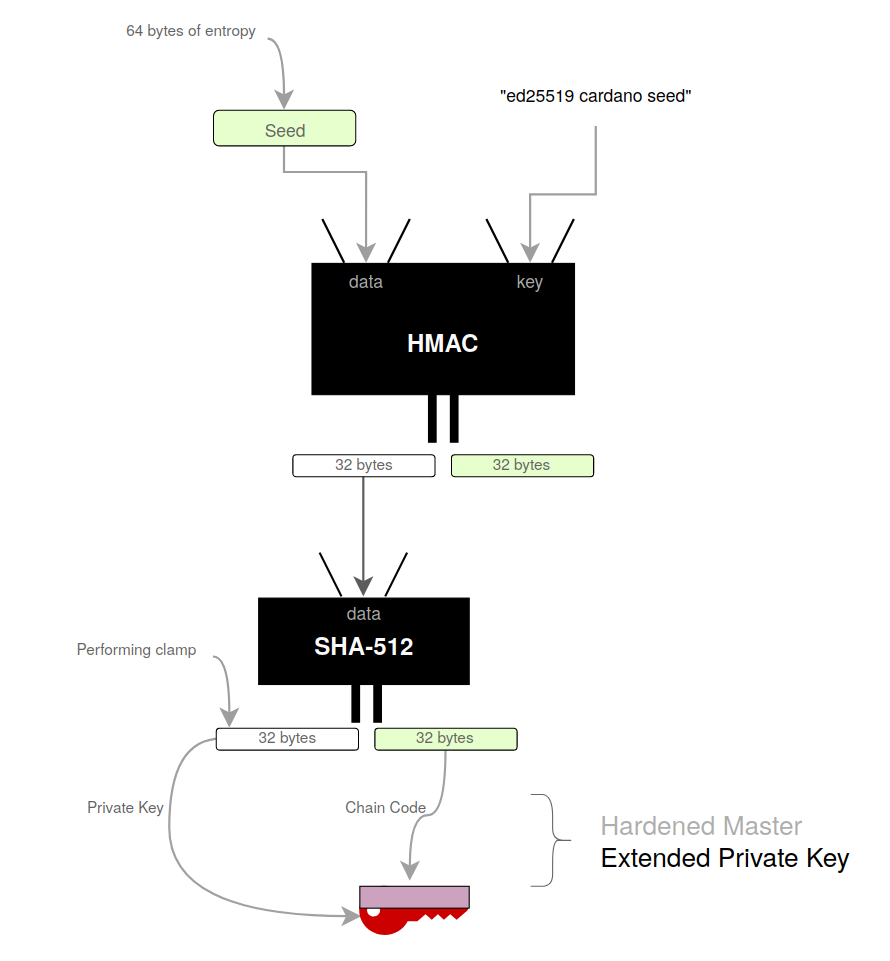
\includegraphics[width=1\textwidth]{images/slip23_master.png}
    \caption[Master key generation process]{Master key generation process}
    \label{fig:slip23_master}
\end{figure}

Pseudo-code:
\begin{enumerate}
    \item Let $S$ be a seed byte sequence such as the master secret from BIP39.
          \begin{quote}
              The length of the seed is from 128 bits to 512 bits.
          \end{quote}
          \bigskip

    \item Calculate $I$ := HMAC-SHA512(Key = ``ed25519 cardano seed", Data = $S$).
          \bigskip
    \item Split $I$ into two 32-byte sequences, $I_L$ as 32 bits left and $I_R$ as 32 bits right.
          \bigskip

    \item Let $k$ := SHA-512($I_L$).
          \bigskip
    \item Split $k$ into two 32-byte sequences, $k_L$ as 32 bits left and $k_R$ as 32 bits right.
          \bigskip
    \item If the third highest bit of $k_L$ (which is $k_L$[29]) is not 0, modify $k$ by assigning:
          \begin{itemize}
              \item $k_L$[0] := $k[0]$ \& 0xf8
              \item $k_L$[31] := ($k_L$[31] \& 0x1f) | 0x40.
                    \begin{quote}
                        This step is compatible with “bit clamping” in Ed25519.
                    \end{quote}
          \end{itemize}
          \bigskip
    \item Let $k_R$ := $k[32:64]$ and use ($k_L$, $k_R$) as the root extended private key and $c$ := SHA-256($I_R$) as the root chain code.
\end{enumerate}

\bigskip
{\textbf{Child key derivation function}}. Surprisingly, BIP32-Ed25519 allows both normal and hardened derivation. We can even generate hardened derivations on public keys since the linearity is ignored. With $B$ is the generator, the next parts will generalize the derivation processes.

\begin{adjustwidth}{0.5cm}{}
    \bigskip
    {\textbf{Private key derivation}}. Let $k$ = ($k_L$, $k_R$) be the extended private key and $K$ the public key. Extended private child key $k_i$ = ($k_L $, $k_R$) for child $i$ is produced as \autoref{fig:slip23_private}.
    \begin{figure}[ht!]
        \centering
        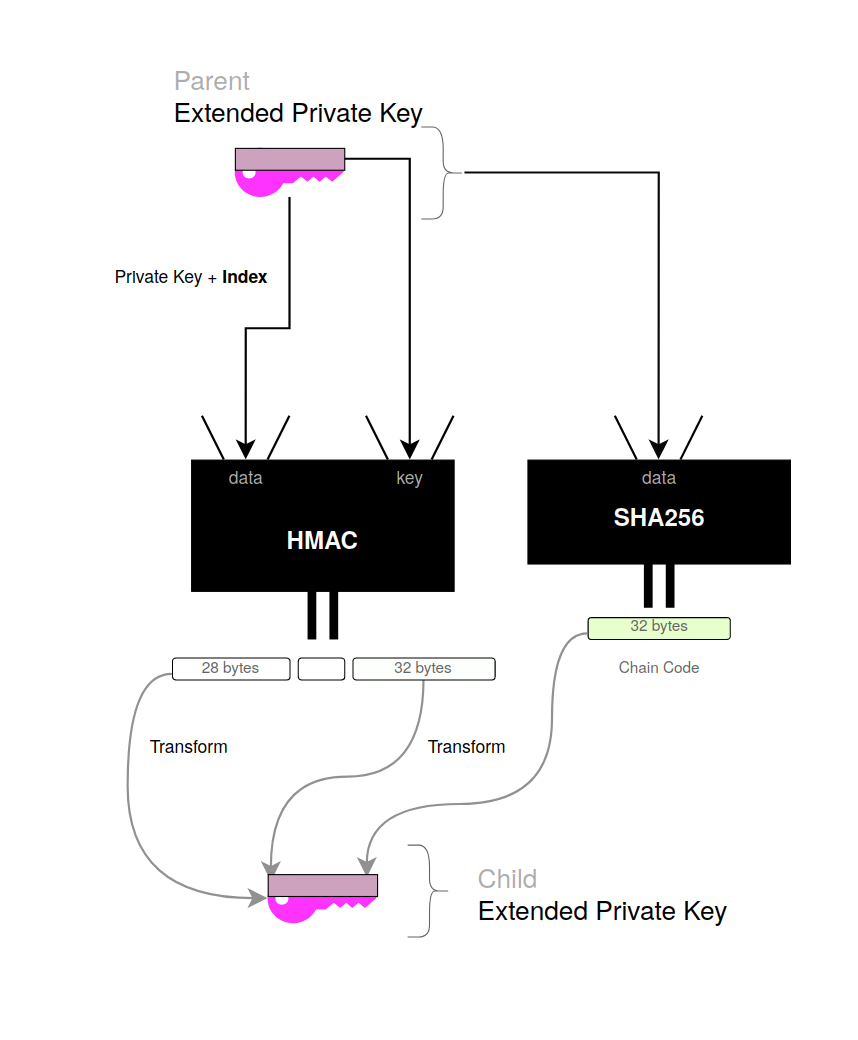
\includegraphics[width=1\textwidth]{images/slip23_private.png}
        \caption[Private keypair derivation process]{Private keypair derivation process}
        \label{fig:slip23_private}
    \end{figure}

    Pseudo-code:
    \begin{enumerate}
        \item Check whether $i \geq 2^{31}$ (whether the child is a hardened key).
              \begin{itemize}
                  \item If so (hardened child):
                        \begin{quote}
                            let $Z$ = HMAC-SHA512(Key = $c_{par}$, Data = 0x00 $\parallel$ $k_{par}$ $\parallel$ $ser_{32}(i)$).

                        \end{quote}

                  \item If not (normal child):
                        \begin{quote}
                            let $Z$ = HMAC-SHA512(Key = $c_{par}$, Data = 0x02 $\parallel$ $ser_{P}(K_{par})$ $\parallel$ $ser_{32}(i)$).

                            The value $ser_P(K_{par})$ is represented as a little-endian string of 32 octets defined in Ed25519 signature \cite{DBLP:journals/rfc/rfc8032}.

                        \end{quote}
              \end{itemize}
              \bigskip

        \item Split $Z$ into two parts: the left 28-byte sequences $Z_L$ and right side 32-byte sequences $Z_R$.
              \begin{itemize}
                  \item let $k_L$ = 8$Z_L$ +  $k_{parL}$. If $k_L$ mod n (base order) = 0: return false.

                  \item let  $k_R$ = $Z_R$ +  $k_{parR}$ (mod 2**256)

              \end{itemize}
              \bigskip

        \item The returned child private key ($k_L$, $k_R$).

              \bigskip
        \item Check whether $i$ $\geq$ $2^{31}$ (whether the child is a hardened key).
              \begin{itemize}
                  \item If so (hardened child):
                        \begin{quote}
                            Return  $c_i$= HMAC-SHA512(Key = $c_{par}$, Data = 0x01 $\parallel$ $k_{par}$ $\parallel$ $ser_{32}(i)$).
                        \end{quote}
                  \item If not (normal child):
                        \begin{quote}
                            Return  $c_i$= HMAC-SHA512(Key = $c_{par}$, Data = 0x03 $\parallel$ $ser_P(K_{par})$ $\parallel$ $ser_{32}(i)$).
                        \end{quote}
              \end{itemize}
              \bigskip
        \item The child public key $K_i$ can be derived as $K_i$ = $k_L$B.

              \bigskip

    \end{enumerate}


    \bigskip
    {\textbf{Public key derivation}}. Same as BIP32, the SLIP32 schema allows us to generate hardened and normal child keys from extended parent keys. \autoref{fig:slip23_public} presents the process of SLIP23 public key derivation.
    \begin{figure}[ht!]
        \centering
        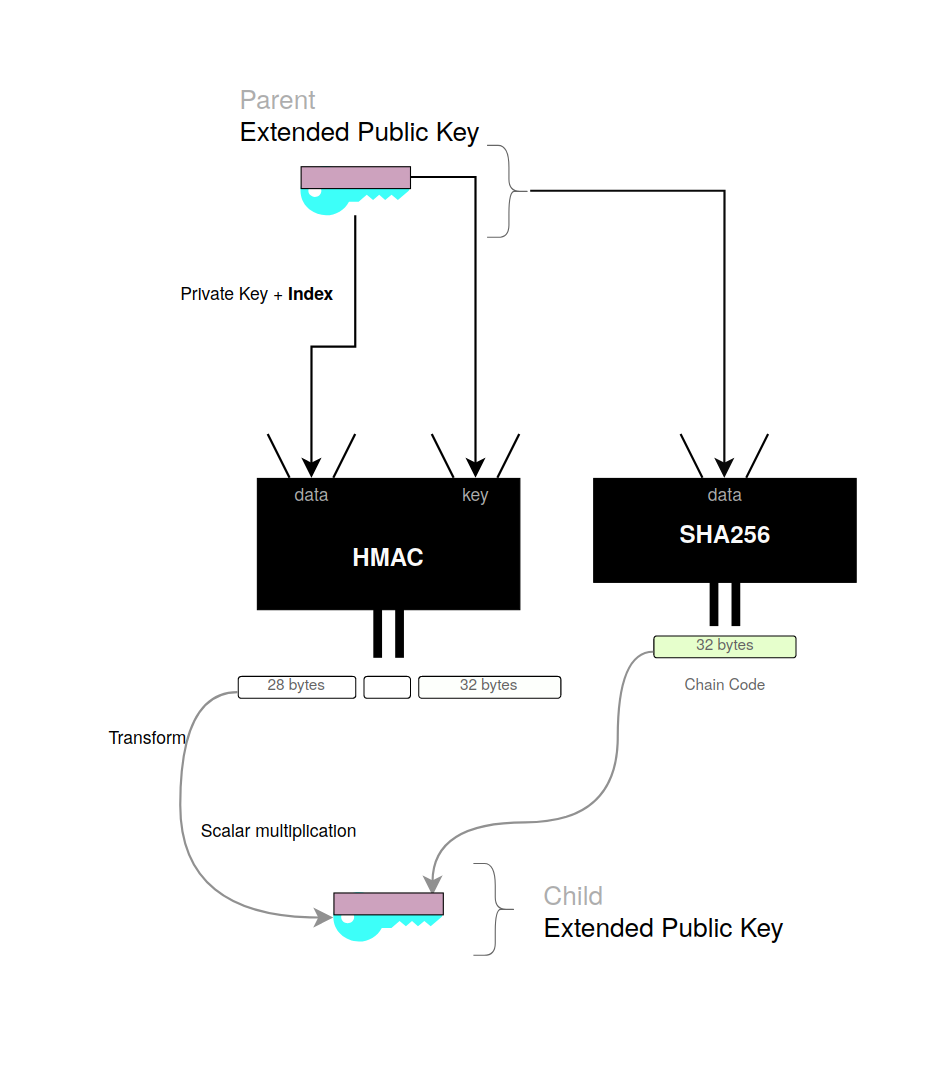
\includegraphics[width=0.9\textwidth]{images/slip23_public.png}
        \caption[Public keypair derivation process]{Public keypair derivation process}
        \label{fig:slip23_public}
    \end{figure}

    Pseudo-code:
    \begin{enumerate}
        \item Check whether $i \geq 2^{31}$ (whether the child is a hardened key).
              \begin{itemize}
                  \item If so (hardened child):
                        \begin{quote}
                            let $Z$ = HMAC-SHA512(Key = $c_{par}$, Data = 0x00 $\parallel$ $k_{par}$ $\parallel$ $ser_{32}(i)$).

                        \end{quote}

                  \item If not (normal child):
                        \begin{quote}
                            let $Z$ = HMAC-SHA512(Key = $c_{par}$, Data = 0x02 $\parallel$ $ser_P(K_{par})$ $\parallel$ $ser_{32}(i)$).

                        \end{quote}
              \end{itemize}
              \bigskip

        \item Split $Z$ into two parts: the left 28-byte sequences $Z_L$ and right side 32-byte sequences $Z_R$. (No usage of  $Z_R$)

              \bigskip
        \item Calculate the child public key $K_i$:
              \begin{quote}
                  $K_i$ = $K_p$ + 8$Z_L$B. If $K_i$ equals to the identity point (0,1) return false.
              \end{quote}

              \bigskip

        \item Check whether $i$ $\geq$ $2^{31}$ (whether the child is a hardened key).
              \begin{itemize}
                  \item If so (hardened child):
                        \begin{quote}
                            Return  $c_i$= HMAC-SHA512(Key = $c_{par}$, Data = 0x01 $\parallel$ $k_{par}$ $\parallel$ $ser_{32}(i)$).
                        \end{quote}
                  \item If not (normal child):
                        \begin{quote}
                            Return $c_i$ = HMAC-SHA512(Key = $c_{par}$, Data = 0x03 $\parallel$ $ser_P(K_{par})$ $\parallel$ $ser_{32}(i)$).
                        \end{quote}
              \end{itemize}
              \bigskip

    \end{enumerate}

    In summary, the above methods allow the derived child private keys to correspond to the child public key. The advantages described in Section \ref{bip32} are enabled.
    The authors gives us an working derivation schema but they didn't explained why did they choose specific metrics for the schema. For example they shortened to 28-byte of $Z_L$ for the child keys.
    The $Z_R$ of public key derivation is completely unused.

\end{adjustwidth}

\bigskip
{\textbf{The BIP32-Ed25519 key leakage problem}}. Same as BIP32, the problem is if the attackers have one of the private child keys, can they recover all of the other wallets? The answer is no thanks to the hash function HMAC-SHA512 between the secret parent key and its children. Therefore, the extended key can be guessed by brute-force 2**256 different master secrets. But the number of recovered wallets is only limited in this case. They can retrieve only the parent keys they derived from and then generate all branches of child keys from that node. This may lead to a fundamental leakage problem if the implementers fail to check the depth of child wallets. The implementers also have difficulties reviewing all the cases, even harder to keep track of the depth when more child wallets are produced. This case raises a problem in our thesis where we allow users (who have no ideas of the security issues) to choose their index and depth of the tree. Hardened derivation of BIP32-Ed25519 also is vulnerable to this attack vector. Furthermore, using the public key as a part of the function to derive a child private key won’t serve the standard properties that the SLIP10 hardened key provided.

\bigskip
{\textbf{The BIP32-Ed25519 bit clamping before signing problem}}. Jeff Burdges (Web3 Foundation, Polkadot Blockchain), who is famous for finding the vulnerabilities in the BIP32-Ed25519 proposal, warned us about a potential attack vector occurring under the many time the derivation function clamping. Ed25519’s bit clamping is only designed for preventing attacks in the signing method and key exchange. According to Burdges, clamping the bits doesn’t make the key more secure; instead, it makes the key weaker. BIP32-Ed25519 also uses only 224-bit scalar derivation (28-byte), so each level of derivation weakens the adequate strength of the computed scalar value.
Burdges also mentioned a straightforward full key recovery attack if one permits long key derivation paths along with either clamping by an Ed25519 library \cite{Jeff}.

In conclusion, there are three most notable key derivation methods that we mentioned. There is some more approach to HD key tree derivation like the Tor’s approach \cite{torspec}. It was released four years before the BIP32-Ed25519. However, they haven’t published any implementations as well as the test vector on the internet, making it very hard for the open-source researcher and the community to validate. We consider any project with this behavior as a fraud proposal and continue with our thesis.

\subsection{BIP39 - Random Password Generator}
\label{bip39}
BIP39 is one of the many design ideas that was approved by an economic majority of the blockchain community and became a standard for many popular wallets. It describes the implementation of a mnemonic sentence (“mnemonic code”, “seed phrase”, “seed words”) -- a group of easy to remember words -- for the generation of deterministic wallets, making it more convenient for humans to store (compared to random raw binary or hexadecimal representations of a wallet seed). A mnemonic sentence is a way of representing a large randomly-generated number as a sequence of words. These words are then used to create a seed S, which can replace the root seed generated from PRNG in the BIP32 or SLIP10 section. The process of creating a random secret key is present in \autoref{fig:bip39}.

\begin{figure}[ht!]
    \centering
    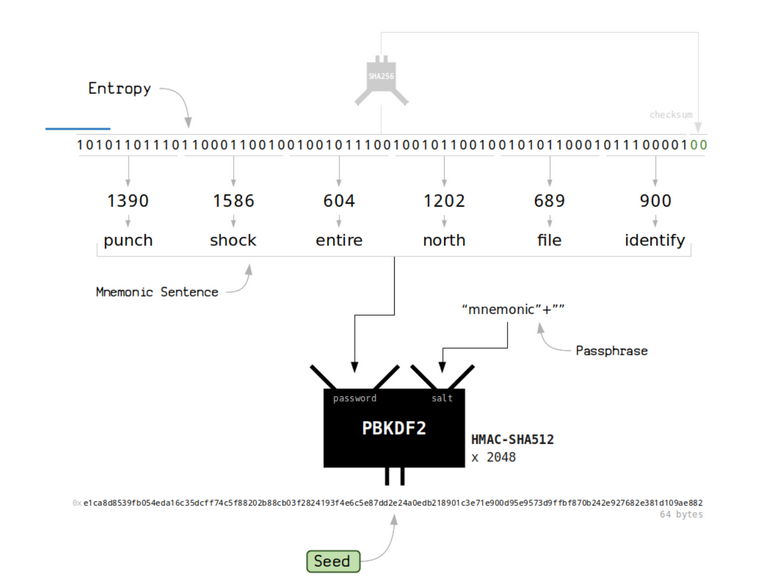
\includegraphics[width=0.9\textwidth]{images/bip39.png}
    \caption[Random secret seed generation process]{Random secret seed generation process \cite{learnme}}
    \label{fig:bip39}
\end{figure}

\bigskip
{\textbf{Generate Mnemonic}}. The first of all steps is to generate entropy, which is our source of randomness. The entropy (ENT) we produce must be a multiple of 32 bits, allowing us to split the entropy up into even chunks and convert to words later on.
The proper size of ENT is 128-256 bits, that’s enough to make it impossible for two people to generate the same entropy.
Entropy values must be sourced from a strong source of randomness. This means flipping a fair coin, rolling a fair dice, noise measurements etc.

Next, create a bit sequence of the SHA256 hash of ENT called checksum where n = ENT.length / 4. This value is appended to the end of ENT. Next, these converted bits are split into groups of 11 bits, each encoding a number from 0-2047, present as an index. Finally, we convert these numbers into words from the BIP39 wordlist and use these words as a mnemonic sentence.

\bigskip
{\textbf{Mnemonic to Seed}}. To create a root seed from the mnemonic, BIP39 uses the PBKDF2 function with the generated mnemonic sentence (in UTF-8 NFKD) used as the password and the string ``mnemonic" + optional passphrase (UTF-8 NFKD) as the salt. The iteration count is set to 2048. The HMAC-SHA512 is used as the pseudo-random function, providing the length of the derived key is 512 bits (64 bytes).


\subsection{BIP44 - Index Path for Multi-coin Wallet}
BIP44 \cite{bip44} defines an index path for key derivation in BIP32, allowing a wallet to handle multiple coins, multiple accounts, external and internal chains per account, and millions of addresses per chain. In BIP44, Bitcoin registers their coin type as 0 and their testnet as 1. Later on SLIP44 \cite{slip44}, other blockchains start to register their type too. Right now there are more than 2000 indexes (each index represents a blockchain) on SLIP44 documentation.

\bigskip
{\textbf{Wallet Structure}}. Each node of structure has a different meaning but we will use BIP44 as a standard path for key derivation. \autoref{fig:bip44_path} presents the initial idea of how BIP 44 path look like.

\begin{figure}[ht!]
    \centering
    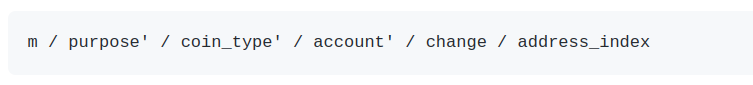
\includegraphics[width=0.9\textwidth]{images/bip44_path.png}
    \caption[Example path of BIP44]{Example path of BIP44}
    \label{fig:bip44_path}
\end{figure}

BIP44 defines a logical hierarchy for deterministic wallets. Each level of the hierarchy has a meaning, describe as follow (see also \autoref{fig:bip44}):

\begin{figure}[ht!]
    \centering
    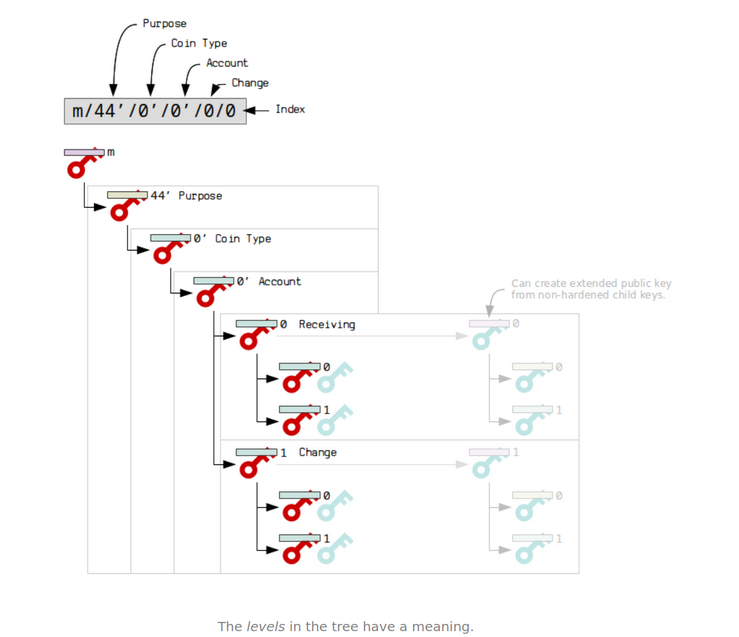
\includegraphics[width=0.9\textwidth]{images/bip44.png}
    \caption[Example tree of wallets from given path]{Example tree of wallets from given path \cite{learnme}}
    \label{fig:bip44}
\end{figure}

\begin{itemize}
    \item \textbf{m (or M)}: The master private key generated from root seed.
    \item \textbf{purpose}: Purpose is set to 44' constant (or 0x8000002C). It meaning that the child keys of this node is used according to BIP44 specification.
    \item \textbf{coin type}: One master secret seed can be used for unlimited number of independent cryptocurrency such as Bitcoin, Solana or Ethereum. However, sharing the same space for various blockchain may has some disadvantages. Creating this level makes sure a separate subtree for every blockchain, avoiding reusing the same addresses across cryptocoins and improving privacy character. Coin type is a constant, set for each blockchain. Blockchain developers will ask for registering an unused number for their blockchain (see \cite{bip44}).
    \item \textbf{account}: An parameter that separate the path for funds. This node splits the key range into independent user identities, so the wallet avoids mixing the cryptocurrency across different accounts. Users can use these wallets to organize the funds in the same fashion as bank; for donation purposes, for saving purposes, for common expenses etc.
    \item \textbf{change}: Constant 0 is used for external chain and constant 1 for internal chain (also known as change addresses). External chain is used for addresses that are meant to be visible outside of the wallet (e.g. for receiving payments). Internal chain is used for addresses which are not meant to be visible outside of the wallet and is used for return transaction change.
    \item \textbf{index}: Addresses are numbered from index 0 in sequentially increasing manner. This number is used as child index in BIP32 derivation.

\end{itemize}


\section{Related Works}
\label{related}

The HD wallets on curve Ed25519 were quite a challenge for the community. There has been quite an effortless number of implemented open-source libraries and evaluated by experts in cryptography. We do not try to find and analyze all applicable works. Instead, we focus on the notable library and the application that is generally used. We divide into two categories as the core library and real-world implementation.

\bigskip
{\textbf{Library implementation}}

The SLIP10 approach is widely used because of its easy understanding process and strict security. \textit{christsim}'s Typescript library \cite{christsim} followed all the instructions of SLIP10 and provided all derivation features of the three curves in SLIP10. However, it lacks test vectors on Ed25519 keys. The code seems to be redundant since using class objects but never making use of OOP structure.

\textit{alepop / ed25519-hd-key} (github) \cite{alepop} offers a simpler implementation of SLIP10 using functional programming. It is only built for Ed25519 key generation. The library provides valid result keys or input path checking and also gives the user permission to change the value of the offset (range of hardened keys).

\textit{chatch / stellar-hd-wallet} is an HD wallet library designed for the Stellar (blockchain) application. It implements full hardened derivation of the SLIP10 version and supports multiple languages for mnemonic code. The library lacks a Stellar address extraction from the public key.

On the other hand, due to the missing references and test vectors, BIP32-Ed25519 struggles with many incompatible implementations.

\textit{vbmirthr}'s OCaml library \cite{vinc} and \textit{islishude}'s Go implementation \cite{Shude} follow BIP32-Ed25519 original master key derivation specification and use SHA512 and SHA256 for deriving the private key k and chain code c (respectively) from the master secret S.

LedgerHQ's Python implementation \cite{LedgerHQ} uses HMAC-SHA512 and HMAC-SHA256 instead.
Furthermore, vbmirthr's instructions to discard the seed (i.e. master secret) if the master key's third-highest bit of the last octet of $k_L$ is not zero. Meanwhile, islishude's Go library just follows BIP32-Ed25519 papers and clears the master key's third-highest bit. LedgerHQ's implementations repeatedly set the seed and feed the input to the master key generation and restart the process until a master key meets the desired properties.


\bigskip
{\textbf{Real-world application}}

Interestingly, the IOTA ledger combines Ed25519 as a second signature scheme with the currently used Winternitz-OTS [Ref] but uses SLIP10 as their key derivation schema.
They aim to address all the points above with the drawback of being less quantum robust. The digital signature is called a bundle, and they prove it is sufficiently immune against a powerful quantum computer running Shor’s algorithm \cite{shor} when addresses are not reused.

Sollet \cite{sollet} is a famous open-source non-custodial and HD wallet for users to manage assets on the Solana blockchain safely. Users can access the wallet by their browser. The wallet provided multiple types of token (only on chain) management. But the user only has access to one wallet at a time. If they want to use another, they will have to log out and choose a different index. The wallet is mainly used by developers for testing.

The Polkadot community recommends their wallet developers implement SLIP10 since they haven’t prioritized investigating into Bip32-Ed25519. Jeff Burdges research on Polkadot wallet security refers to BIP32-Ed25519 as a “zombie” \cite{Jeff1} and suggests their cryptosystem should not use this as HD wallet core.

Oasis \cite{oasis} on the other hand don't use use BIP32-Ed25519's private and public key directly but use the obtained $k_L$ (first 32 bytes) of the 64 byte BIP32-Ed25519 derived private key as Ed25519's seed (i.e. non-extended private key). But in Mar 2021 they decided to change from BIP32-Ed25519 to SLIP10 schema, leaving it “not applicable in future”.

The BIP32-Ed25519 has been very poorly adapted in practice ever since Jeff Burdges's warning \cite{Jeff}. But it is still very useful for cold wallets. Hardware wallets \href{https://www.ledger.com/}{Ledger} and \href{https://trezor.io/}{Trezor} implement both SLIP10 and BIP32-Ed25519 to their key generation schema. The advantages of public-key derivation impactfully remain. Attacks aim to steal private keys from hardware wallets but are still shallow. Users can publish their master public key to the networks, while child keys can be kept safe in users' pockets. If ever the transaction is needed, users just need to derive child keys from their hardware and sign the transaction. Plus, Ledger and Trezor are better than other wallets since they are custodial type wallets and can hold multiple types of native tokens.

